\chapter{Lösungsentwicklung}
\label{cha:Lösungsentwicklung}

\section{Das System}
\label{cha:Das System}

Die entwickelte DAPP ermöglicht es einem Owner ein Objekt über die Blockchain zu vermieten. Er kann dabei das Depot und die Mietkosten festlegen. Ein Renter kann dann dieses Objekt für eine bestimmte Zeit mieten. Die Abwicklung des Vertrages und dessen Kosten geschieht im Hintergrund in der Blockchain. Es gibt keinen Zwischenmann (z.B. Bank), der für die Überweisung zuständig ist, sondern das Geld fliesst direkt vom Renter zum Owner. 
Ein Objekt kann grundsätzlich alles sein: Ein elektrisches Fahrrad, eine Ferienwohnung oder einfach ein Schließfach. Es muss jedoch möglich sein ein Kontrollmechanismus anzubringen, der gleichzeitig ein Node in der Blockchain darstellt. Bei einem elektrischen Fahrrad wäre es z.B. möglich einen Minicomputer im Fahrgestellt zu montieren, welcher den Akku aktiviert oder deaktiviert und über eine Sim-Karte mit der Blockchain synchronisiert. Möchte ein Benutzer das Fahrrad verwenden, so müsste er dieses zuerst über die Blockchain mieten und erst dann kann er den Akku aktivieren. Die Mietkosten würden direkt dem Anbieter des Fahrrades überwiesen werden.

\vspace{1em}
Als Proof of Concept wurde in dieser Arbeit einen Demonstrator entwickelt. Es handelt sich um ein Schliessfach-Vermietsystem, welches als Backend eine private Blockchain nutzt. Jedes Fach hat ein elektrisches Türschloss, welches über ein Raspberry PI durch die Blockchain kontrolliert wird. Ein Schließfach und ein Raspberry PI bilden zusammen eine Einheit (ein Node der privaten Blockchain). Das erste Schliessfach erstellt ausserdem ein WLAN Hotspot, auf den alle anderen Einheiten verbinden. Der Demonstrator verfügt über 3 Einheiten, welche sich zum Hotspot verbinden. Die Anzahl der Einheiten ist nicht beschränkt, solange sie in der Reichweite des WLAN Hotspots befinden. Alle Einheiten zusammen bilden die private Blockchain. 

\subsection{Interaktion mit dem Demonstrator}
Ein Benutzer muss sich zuerst als einen weiteren Node mit der Blockchain verbinden. Anschliessend kann er über die entwickelte Webapp (DAPP) mit dem System interagieren. 

\vspace{1em}\noindent
Folgende Interaktionen sind möglich.

\vspace{1em}\noindent
\textbf{Als Owner}
\begin{itemize}
    \item Neues Rentable (Objekt) erfassen
    \item Bestehende Rentable deaktivieren/aktivieren/zerstören
\end{itemize}

\vspace{1em}\noindent
\textbf{Als Renter}
\begin{itemize}
    \item Nach Rentables suchen (Discover)
    \item Informationen und Verfügbarkeit eines Rentables prüfen
    \item Ein Rentable reservieren (rent)
\end{itemize}

\vspace{1em}\noindent
\textbf{Als aktueller Renter (current renter)}
\begin{itemize}
    \item Sperren und Entsperren des Rentables (Lock/Unlock)
    \item Zurückgeben des Schließfachs (Unclaim)
    \item Verlängern der aktuellen Reservation (Emergency)
\end{itemize}

\subsection{Regeln}
\begin{enumerate}
    \item Hat zum aktuellen Zeitpunkt niemand das Rentable reserviert, so ist der Owner gleich dem Renter.
    \item Es gibt keine Reservationsüberlappungen
    \item Eine aktive Reservation kann mittels \emph{Emergency} verlängert werden. Steht die Verlängerung im Konflikt mit einer nächsten Reservation, so wird der Startzeitpunkt der Reservation nach hinten verschoben. Wird im Fallbeispiel ... erläutert.
    \item ...
\end{enumerate}


\subsection{Fallbeispiele}

\subsubsection{Normal-Fall}
Der Benutzer A reserviert das Schliessfach von tR1 bis tR2 zum Zeitpunkt t0. Das Deposit und die Mietkosten werden ihm somit abgezogen.
Zum Zeitpunt tR1 wird Benutzer A zum \emph{Current Renter} und besitzt dadurch privilegierten Zugriff. Er kann jetzt das Schliessfach öffnen (Unlock) und schliessen (Lock). Nach einer gewissen Zeit noch vor Ablauf der Reservation, entschliesst sich Benutzer A das Schliessfach wieder abzugeben (Unclaim), da er es nicht mehr benötigt. Die Reservation wird somit auf diesen Zeitpunkt gekürzt und Benutzer A erhählt sein Deposit und die Mietkosten für die ungenutzte Zeit zurück. Die priviligierten Rechte werden umgehend wieder an den Owner abgegeben.

\subsubsection{Reservationsende ohne Betätigung der Rückgabe}
Wie im Normal-Fall beschrieben, ist Benutzer A momentaner Renter (current renter) des Schliessfaches. Anstelle jedoch das Schliessfach wieder zurückzugeben lässt er die Reservationszeit auslaufen. Zum Zeitpunkt tR2 werden ihm die Rechte entzogen er erhält keine Rückerstattung des Deposits. Es liegt also in Benutzer A seinem Interesse, alle eingeschlossenen Gegestände vor Ablauf der Reservation aus dem Schließfach zu nehmen und dieses Zurückzugeben (Unclaim).

\subsubsection{Verlängern der Reservationsdauer}
Der Benutzer A sollte immer einen Buffer in die Reservationszeit einplanen, damit er das Schließfach auch noch bei Zugsausfall oder einem Autounfall rechtzeitig vor Reservationsablauf erreichen kann. In äußersten Notfällen kann es trotzdem vorkommen, dass der Benutzer A nicht rechtzeitig seine Affären aus dem Schließfach nehmen kann und aus diesem Grund hat er die Möglichkeit eine \emph{Emergency} auszulösen. Die Emergency ist entsprechend kostenintensiv und sollte deswegen nur in Notfällen und abhängig vom Wert der Gegenstände im Schließfach in Erwägung gezogen werden. 
Die Emergency verhindert den Ablauf der aktuellen Reservation und überschreibt allenfalls nachfolgende Reservationen. Betroffene Reservationen erhalten einen Teil der Einnahmen durch die Emergency als Entschädigung.

\subsubsection{Fall von Schäden}
Benutzer A reserviert wie im Normal-fall ein Schliessfach. Zum Zeitpunkt t1 will er das Schliessfach öffen (Unlock), dieses reagiert jedoch nicht. Er muss nun Kontakt mit dem Owner aufnehmen und die Sache klären. Auf jeden Fall sollte er nun das Schliessfach zurückgeben (Unclaim) um die Kosten niedrig zu halten, im Falle, dass sich der Owner nicht auffinden lässt oder dieser kein Interesse zeigt.

Im Rahmen dieser Arbeit wurde auch ein Konzept überlegt, wie solche Probleme vermindert werden könnten. Durch Einführen eines Review Systems, wo Benutzer die Owner beurteilen können. Owner mit einer guten Bewertung (Score) wären dann vertrauenswürdiger.

\begin{itemize}
    \item \textbf{ Wie funktioniert unsre Loesung? }
    \item \textbf{ Was ermoeglicht unsere Loesung? }
    \item \textbf{ Wie sicher ist das System? }
    \item \textbf{ Was sind moegliche Angriffe? }
    \item \textbf{ Wie stehts mit der Verfuegbarkeit?}
    \item \textbf{ Gibt es Restrictions?}
    \item \textbf{ Was sind die Staerken und Schwaechen dieser Loesung? }
    \item \textbf{ Wie ist der Ablauf? Was geschieht wann?}
    \item \textbf{ Was kann der Benutzer machen?}
    \item \textbf{ Wie sind die Regeln? Wer kann reservieren und wann? Was passiert, wenn die Reservation ablauft? Wer haftet? Was ist, wenn das Schliessfach beschaedigt ist und ich es nicht antreten kann?}
    \item \textbf{ Wie sieht das Kostenmodel aus? Beispiele und Scenarien?}
    \item \textbf{ Wer nutzt unsere Loesung? }
    \item \textbf{ Warum nutzt man unsere Loesung?}
    \item \textbf{ Was sind Scenarien, wo unsere Loesung zum einsatz kommen wuerde?}
    \item \textbf{ Wie ist der grobe Aufbau?}
    \item \textbf{ Was fuer Technologien setzen wir ein und weshalb Blockchain?}
    \item \textbf{ Wie ist die Interaktion mit dem Benutzer? Kontextdiagramm? Es gibt mehrere Benutzer und Rollen.}
    \item \textbf{ Was brauchts um diese Loesung um zu setzten? Smart Contracts, Blockchain, Hardware, WebUI }
    \item \textbf{ In welche Komponenten ist das System aufgeteilt. Was sind die eizelnen Funktionen?}
    \item \textbf{ Was sind die Abhaengikeiten unseres Systems?}
    \item \textbf{ Wie sehen die Schnittstellen aus?} 
    \item \textbf{ Was fuer Technologien werden eingesetzt?} 
    \item \textbf{ Wie sieht das Design der Komponenten aus? Erweiterbar? Wartbar?} 
    \item \textbf{ Wie sieht das User Interface aus?} 
    \item \textbf{ Welche Libraries verwenden wir? Was haben wir entwickelt?}
    \item \textbf{ Wie wird das System deployed?}
    \item \textbf{ Kann man updates fahren?}
    \item \textbf{ Schrittanleitung zur Installation?}
\end{itemize}
    
    
\begin{figure}
\centering
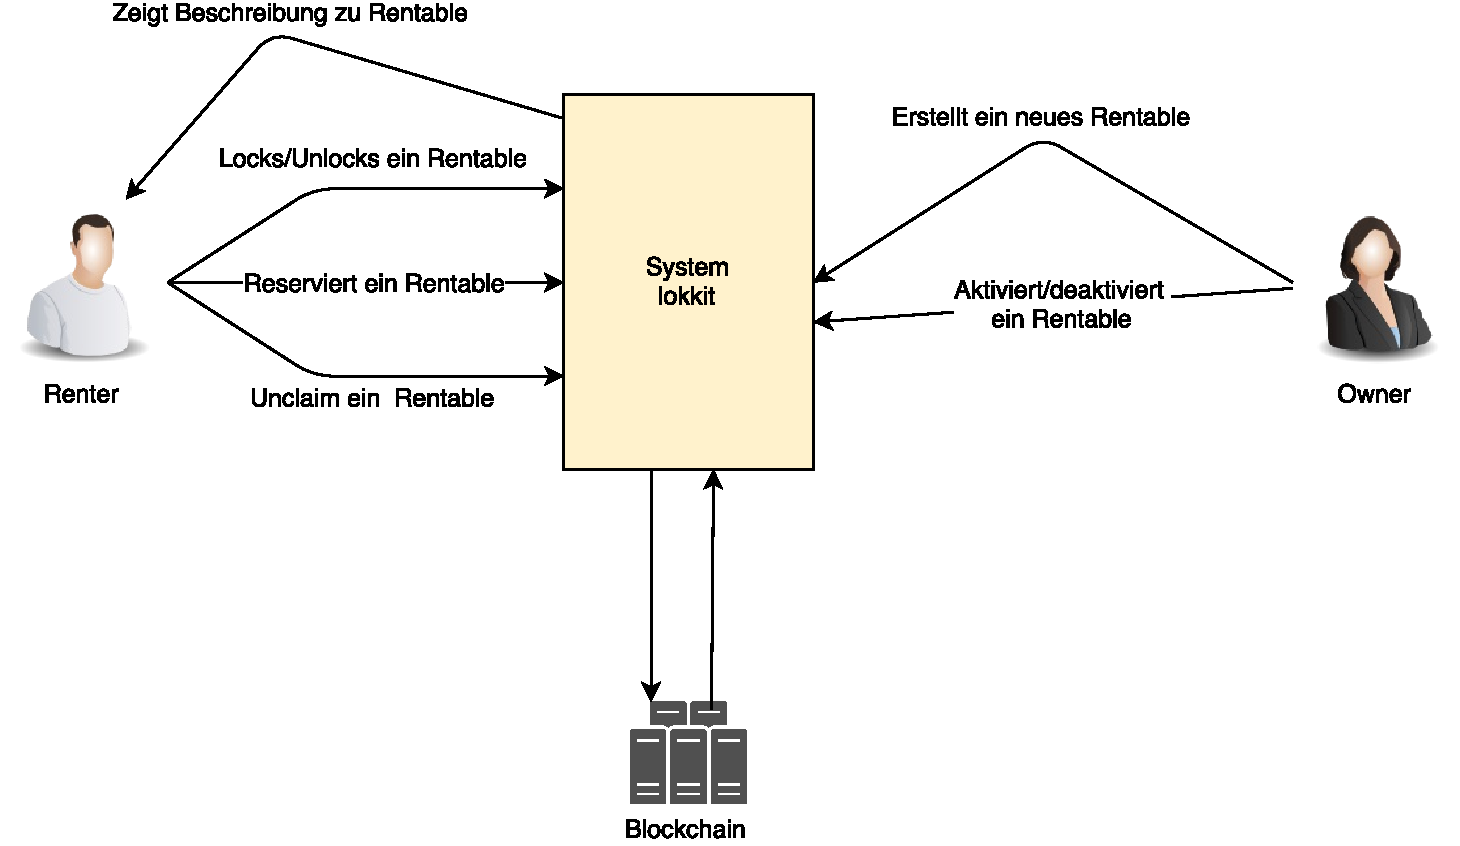
\includegraphics[width=.95\textwidth]{Kontext_Diagram}
\caption{Kontextdiagramm}
\label{fig:Aufbau Komponenten und Schnittstellen}
\end{figure}
Um eine Lösung zu dieser 

\section{Arbeitsmethodik}
\begin{itemize}
    \item \textbf{Wie ist das Projekt abgelaufen?}
    \item \textbf{Was wurde erreicht? Was nicht?}
\end{itemize}
Da in diesem Projekt eine konkrete Aufgabenstellung selbst zu erarbeiten war, und keine konkreten, lieferbaren Objekte vorgesehen waren, wurde zu Beginn eine explorative ad-hoc Methodik verfolgt. Dabei wurde im Projektteam wöchentlich der bisherige Fortschritt analysiert und weitergehende Schritte besprochen. So wurde gewährleistet, dass in der Anfangsphase eine geeignete Aufgabenstellung gefunden werden kann.
\par
Sobald die Aufgabenstellung gefunden wurde, wurde in ein iterativ- inkrementelles Modell gewechselt. Die wöchentlichen Besprechungen wurden beibehalten, um den Fortschritt des Produkts zu verfolgen.

\section{Systemübersicht IoT}
\label{sec:Setup_IoT}
Übersicht: Raspis, Schliessfächer etc...
\begin{figure}
\centering
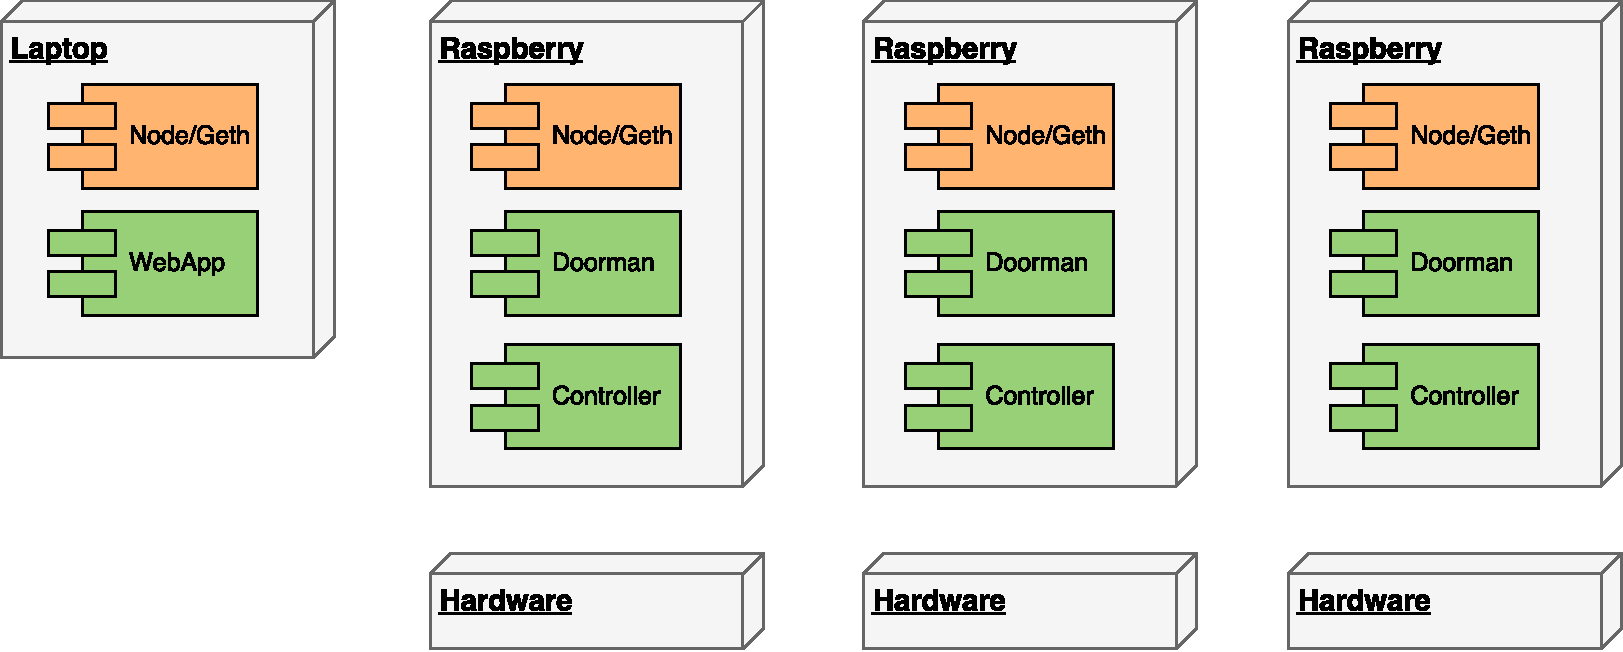
\includegraphics[width=.95\textwidth]{Aufbau_Komponenten}
\caption{Komponenten und Schnittstellen}
\label{fig:Aufbau Komponenten}
\end{figure}
\subsection{Systemkontext}

\subsection{Systemkomponenten}

\begin{figure}
\centering
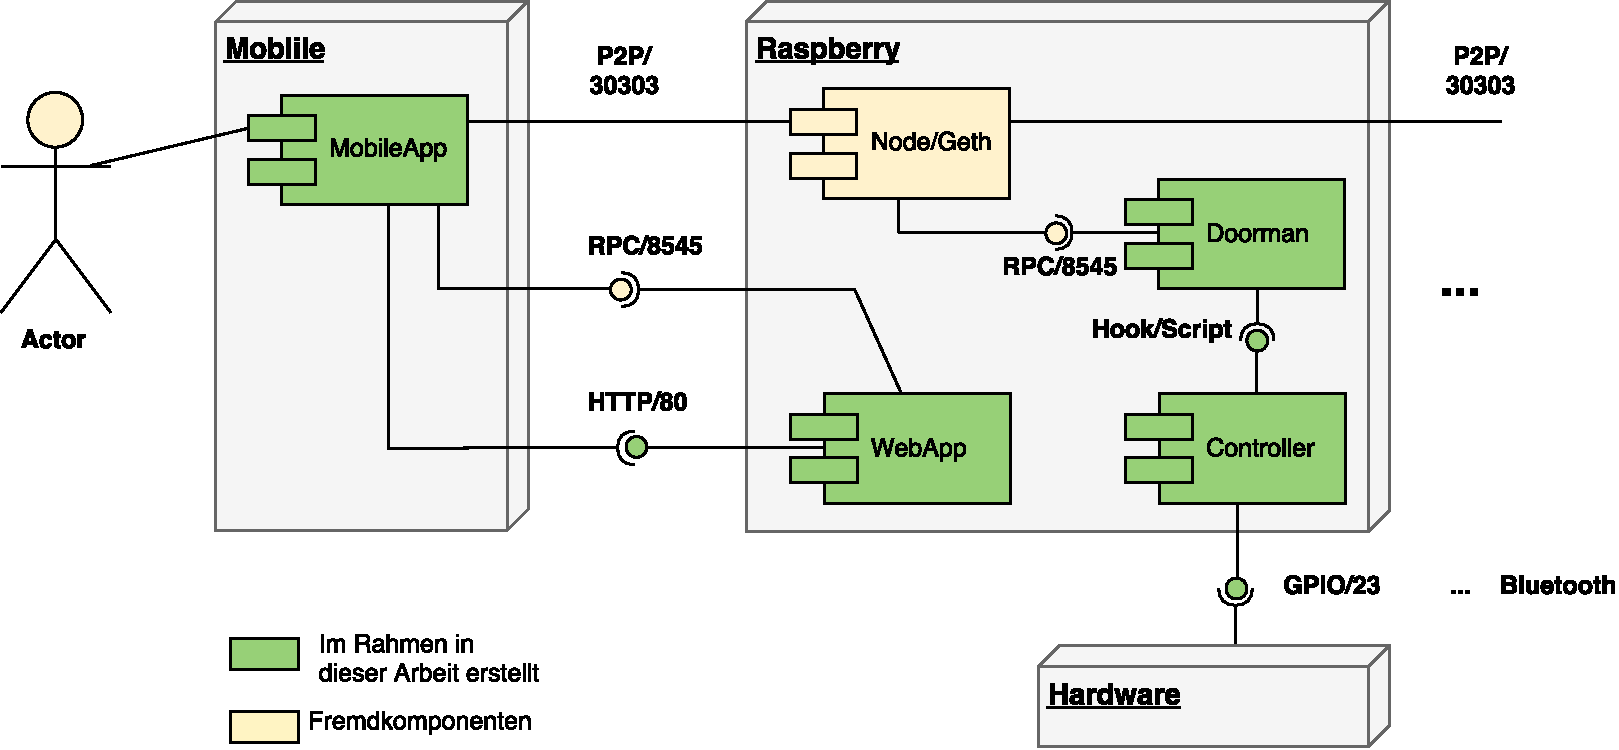
\includegraphics[width=.95\textwidth]{Aufbau_Komponenten_Interface}
\caption{Komponenten und Schnittstellen}
\label{fig:Aufbau Komponenten und Schnittstellen}
\end{figure}



\section{Blockchain}
\label{sec:Blockchain}
referenz, verweise

\subsection{Verwendete Implementation}
Dieses Projekt verwendet die open-source Blockchain-Implementation Ethereum\footnote{https://www.ethereum.org/} als Platform für die Datenhaltung, Erstellung der Business Logik, in Form von Smart Contracts (vgl. \ref{subsec:Smart_Contracts}), und einzige Interaktionsmöglichkeit für Benutzer.\\Ethereum die einzige Implementation einer Blockchain, die zm Start dieses Projektes eine funktionsfähige Plattform für eine Kryptowährung und Smart Contracts zur Verfügung stellt. Weitere Technologien, die in der Evaluationsphase anallysiert wurden, sind Hyperledger, Tendermint und Bitcoin.

\subsubsection{Ethereum}
Die Entwicklung der Ethereum Platform durch finanierung durch ein Crowdfunding Projekt im Sommer 2014 gestartet. Der erste Release war ca. ein Jahr später am 30. Juli 2015. Für die Implementation des lokkit Demonstrators wurde die aktuellste Version des Ethereum Protokolls, mit Namen Homestead, verwendet.
\paragraph{Konsensus}
Alle bisherigen Versionen des Ethereum Protokolls (Olympic, Frontier und Homestead) verwenden den \emph{Proof of Work} Algorithmus Ethash\footnote{https://github.com/ethereum/wiki/wiki/Ethash}, um Konsensus zu erreichen. Dies bedeutet, dass für jede Transaktion eine grössere Berechnung (proof) durchgeführt werden muss, bevor die Transaktion an Nachbarnodes mitgeteilt werden und offiziell in die Blockchain eingetragen werden kann. \\Zukünftige Implementationen des Ethereum Protokolls werden voraussichtlich als Konsensusalgorithmus einen \emph{Proof of Stake} Algorithmus verwenden\footnote{}. Grund dafür ist, dass die Kosten, die Blockchain anzugreifen (bspw. um gewisse Blöcke neu zu schreiben durch erneute Berechnung der Hashes und zugehörigen Nonces) zusammen mit den Betriebskosten wachsen\footnote{https://www.coinmanual.com/proof-stake/}\footnote{https://en.bitcoin.it/wiki/Proof_of_Stake}. Folglich kann ein Hochsicherheitssystem, wie es für Finanzdienste wie Banken oder Treuhänder benötigt würde, nur durch sehr hohe Betriebskosten realisiet werden.

\paragraph{Solidity}
Auf der \acrfull{EVM} werden mehrere Programmiersprachen angeboten, um Smart Contracts zu verfassen. \#TODO. Solidity ist die neuste Sprache und soll alle bisherigen ablösen\footnote{}.
\paragraph{Whisper}
Whisper, auch analog zu der öffentlichen API \emph{shh} genannt, ist ein Kommunikationsprotokoll für \acrfull{DAPPs}. Nachrichten, die über das Whisper Protokoll verschickt werden, benutzen ebenfalls Ethereum Nodes, lösen aber keine Transaktionen auf der BLockchain aus. Sie werden mit einem timeout (ttl) und topics versehen, die es vereinfachen, diese Nachrichten zu filtern. Wie auch die Transaktionen werden die Whisper Messages an alle Teilnehmer gesendet (broadcast). Beim senden kann ein Absender und Empfänger angegeben werden. Diese dienen dazu Inhalte an Whisper Identities zu senden (\#TODO ist der inhalt für den empfänger verschlüsselt?).

\subsubsection{Hyperledger}
Hyperledger ist ein Unterfangen mehrerer internationaler Firmen (\#TODOLinux Foundation, IBM, Intel etc), das zum Ziel hat, wichtige Funktionalität im Bereich von Blockchains zu erforschen und definieren, um schlussendlich einen industrieweiten offenen Standard für verteilte Ledgertechnologien zu erschaffen\footnote{https://wiki.hyperledger.org/community/welcomesheet}.
\\Zum Zeitpunkt des Starts dieses Projekts waren die Projekte 
\paragraph{Fabric}
\paragraph{Chaintool}

\subsection{Testchain}

\subsection{Private chain mit Ethereum}


\subsection{Smart Contracts}
\label{subsec:Smart_Contracts}
\epigraph{''A computerized transaction protocol that executes the terms of a contract.``} \cite{BlockchainRevolution}
\\Mit diesem Zitat kann grob das Ziel von Smart Contracts beschrieben werden. Verträge, die in einem maschinenlesbaren Format verfasst sind, können mit unmissverständlicher Präzision und ohne Interpretationsspielraum definiert werden. So ist es möglich, einen deterministischen, digitalen Vertrag zu verfassen.
Entgegengesetzt ist es nahezu unmöglich eine Menge von Smart Contracts angesichts einer unüblichen Situation deterministisch abzuarbeiten. -> http://www.ibtimes.co.uk/pwc-blockchain-expert-pinpoints-sources-ambiguity-smart-contracts-1575778

\susubsection{Erstellen}
Um einen Smart Contract zu erstellen, wird mittels einer geeigneten Programmiersprache dieser formell definiert. Dieser geschriebene Programmcode kann mittels einer Transaktion in die Blockchain eingesetzt werden, wobei Initialwerte angegeben werden. Man sprich hierbei vom erstellen einer Instanz des Smart Contracts, ähnlich wie in der objektorientierten Programmierung. Bei der ausgelösten Transaktion gilt es zu beachten, dass diese keinen Empfänger hat; der Empfänger dieser Nachricht ist die Blockchain selbst. Wie bei jeder Transaktion eine gewisse Menge gas mitgegeben werden, damit die Operation abgeschlossen werden kann. Wenn der Code in die Blockchain eingesetzt wurde, erhält diese Instanz des Contracts eine Adresse, über die später mit dieser spezifischen Instanz interagiert werden kann.
Beim Erstellen eines Smart Contracts wird auch ein abi generiert. Dieses beschreibt die möglichen verfügbaren Attribute des Contracts und die Interaktionsmöglichkeiten (\#VGL. Funktionen) inklusive deren allfällige Parameter und Rückgabewerte (\#VGL. Interfacedeklaration in OO Sprachen).

\susubsection{Lesezugriff}
Um ein Attribut auszulesen oder eine Funktion mit konstantem Rückgabewert auszuführen, kann diese über ein verfügbares Interface, wie die JavaScript console von geth, direkt aufgerufen werden. Bei Funktionen mit konstantem Rückgabewert ist zu beachten, dass diese nur auf der lokalen Node emuliert werden (CITATION NEEDED) und es somit nicht möglich ist, eine Änderung in der Blockchain zu bewirken. Diese Funktionen haben folglich nur Lesezugriff.

\subsubsection{Schreibzugriff}
Wenn eine Funktion auf der Instanz aufgerufen wird, die eine Änderung in der Blockchain bewirkt, muss eine Transaktion ausgelöst werden. Der Sender der Transaktion muss dabei für die Kosten für gas und allfällige weitere Kosten (\#VGL. Bezahlbare Funktionen) aufkommen. Der Sender kann nicht nur ein Account sein, sondern auch ein weiterer Smart Contract, an dessen Adresse genügend Ether liegt, um die Transaktionskosten zu begleichen.

\paragraph{Bezahlbare Funktionen}
Einige Funktionen benötigen mehr Ether als nur die gas-Kosten. Wenn beispielsweise eine Dienstleistung oder Sache über einen Smart Contract verkauft werden soll, muss noch eine Menge Ether als Zahlungsmittel überweisen werden. Die Menge Ether ist im Smart Contract festgelegt und kann durch Inspektion des Programmcodes eingesehen werden. Sollte der Kunde zu wenig Ether schicken, kann der Smart Contract definieren, dass die Transaktion nicht erfolgreich ist und der Kunde sein Geld zurückerhält. Dazu kann die Transaktion selbst als nichtig erklärt werden und es muss nicht auf das Withdrawal Muster zuückgegriffen werden.

\subsubsection{Solidity}
Solidity ist eine Programmiersprache zur Erstellung von Smart Contracts auf der \acrfull{EVM}, die syntaktisch stark an JavaScript angelehnt ist. Sie kann auch auf anderen Blockchain Platoformen (wie Tendermint oder Counterparty für Bitcoin) verwendet werden. -> https://www.cryptocoinsnews.com/counterparty-brings-ethereum-smart-contracts-to-the-bitcoin-blockchain/\\Solidity wird, in Anlehnung auf den Ausdruck object-oriented, als contract-oriented beschrieben, da die erstellenden Konstrukte in der Sprache als ''contract`` und nicht ''object`` bezeichnet werden. Inhaltlich beziehen sich die beiden Ausdrücke auf dasselbe Konzept.

\subsubsection{Gängige Muster - GEHÖRT DAS INS KAPITEL "SMART CONTRACTS" ODER HIERHIN?}
Folgend werden einige Muster aufgelistet, die beim Entwurf und der Implementation von Smart Contracts mit Solidity, aufgrund der inhärenten Architektur der Platform und Sprache, beachtet werden sollten. Diese Muster dienen als Richtlinie und umgehen bekannte Limitationen oder schliessen Sicherheitslücken. Es ist möglich unter Misachtung der Muster Smart Contracts zu entwickeln. -> \#ALLE BEISPIELE VON http://solidity.readthedocs.io/en/develop/
\#Alle folgenden Beispiele waren für die Erarbeitung der Rentable \& RentableDiscovery Contracts zu beachten!

\paragraph{Generell}
Instanzen von Smart Contracts erhalten, wie Accounts, ebenfalls eine Adresse, an die Ether geschickt werden kann. Meistens wird dies in Form von Funktionsaufrufen gemacht, allerdings kann auch direkt an einen Smart Contract Ether überwiesen werden. Hierbei ist es wichtig zu beachten, dass der Ether zurückerstattet wird, der aus Veresehen an diesen gesendet wurde (\#VGL Withdrawal Muster).

\paragraph{Withdrawal Muster\footnote{http://solidity.readthedocs.io/en/develop/common-patterns.html\#withdrawal-from-contracts}}
Wenn aus einem Smart Contract eine Transaktion an eine Adresse gestartet wird, muss das gas dafür vom digitalen Vertrag bezahlt werden (oder besser: vom Account, der die ursprüngliche Transaktion an den ersten digitalen Vertrag gestartet hat). Im Fall einer einfachen Überweisung fallen keine gas-Kosten an. Ist das Ziel aber ein anderer Smart Contract, besteht die Möglichkeit, dass der Zielvertrag Code ausführt, wenn er eine Transaktion erhält. Das Withdrawal Muster wird folglich verwendet, um zu verhindern, dass der Quellvertrag dies überprüfen muss oder für die gas-Kosten des anderen Smart contracts aufkommen muss.

Wird das Withdrawal Muster angewendet, überweist ein Smart Contract Ether nicht direkt an eine Zieladresse. Stattdessen merkt er sich die Menge, die einer Zieladresse zusteht und stellt die Möglichkeit zur Verfügung, dass diese Begünstigten Ether abheben können. Dies findet mittels einer Transaction statt, die vom Begünstigten ausgelöst werden muss. Die gas-Kosten für diese Art Funktionen sind meist vernachlässigbar und werden durch die zurückerhaltene Menge Ether kompensiert. Da der Begünstigte die Adresse des Quellvertrags kennt und den Quellcode von Smart Contracts öffentlich ist, kann die Zieladresse sicher gehen, beim aufrufen dieser withdrawal-Funktion auf dem Quellvertrag auch tatsächlich die Menge Ether zurückzuerhalten.


\#möglicherweise ein bildli zeichnen oder beispielcode einfügen


\paragraph{Re-Entrancy}\footnote{http://solidity.readthedocs.io/en/develop/security-considerations.html\#re-entrancy}
Hierbei handelt es sich um ein Muster, das angewendet wird, wenn in einem Smart Contract A ein interner Zustand existiert, der die Menge an Ether speichert, der \emph{anderen} zusteht und eine Möglichkeit besteht, diese Menge Ether zu entnehmen (\#VGL. Withdrawal Muster). Beispiele für zurückzuerstattenden Ether kann ein Gebot in einer Auktion sein oder Depots wie bei lokkit.
Unter der Annahme, dass die Zieladresse für die Rückerstattung ein Smart Contract B ist, kann B A angreifen. Bei einer Transaktion wird immer der zugehörige Code ausgeführt. Das heisst, dass B auf eine eingehende Transaktion reagieren kann und ihrerseits erneut die Transaktionsfunktion von A aktivieren kann (\#VGL. Withdrawal Muster). Wenn der Zustand von A noch nicht geändert wurde, wird der Betrag erneut gesendet, bis A kein Ether mehr zur Verfügung hat.

Um mehrfaches Überweisen von Ether zu verhindern, ist es unvermeidbar, zuerst den internen Status des Vertrags zu ändern, bevor Ether überwiesen wird. Die \emph{total} zur Verfügung stehende Menge Ether eines Smart Contracts wird in der Blockchain gehalten und ist Teil des Konsensus. Es ist somit nicht möglich, dass mehr Ether ausgegeben wird als in dem jeweiligen digitalen Vertrag vorhanden ist. 

In folgendem Beispiel kann die \emph{send} Anweisung in Zeile zwei mehrmals ausgeführt werden, da das deposit erst zurückgesetzt wird, sobald die Übertragung erfolgreich war.
\begin{lstlisting}[language=javascript,caption=fehlerhaftes Code Snippet]
    function withdraw() {
        if (msg.sender.send(deposit[msg.sender])) {
            deposit[msg.sender] = 0;
        }
    }
\end{lstlisting}

// folgende Zeile wehrt die Re-Entrancy Attacke ab, da der interne Kontostand zurückgesetzt wird, die Transaktion ausgelöst wird.
Nachfolgend bewirkt die dritte Zeile, dass der interne Kontostand zurückgesetzt wird, bevor die verfügbare MEnge Ether überwiesen wird.
\begin{lstlisting}[language=javascript,caption=empfohlenes Code Snippet]
    function withdraw() {
        var currentRefund = deposit[msg.sender];
        
        deposit[msg.sender] = 0;
        msg.sender.transfer(currentRefund);
    }
\end{lstlisting}

\section{Komponenten}
\label{sec:Komponenten}
Nachfolgend werden die einzelnen Komponenten beschrieben, die für die volle Funktionalität der lokkit-Philosophie benötigt werden.
\subsection{Doorman}
Doorman implementiert die IoT-Seite der Benachrichtigungen mittels Whisper Protokoll.
\subsubsection{Wieso Python? Wieso Python 2.7?}
\subsubsection{Mechanismus}

\subsection{Smart Contracts (Business Logik)}
Die Smart Contracts, die mit Solidity implementiert wurden, werden nachfolgend erläutert. Diese Implementationen bilden das Rückgrat der Applikation. Sie bilden die Business Logik in Code Form ab und dienen als Zugriffsschicht der Userinteraktion auf die Blockchain als Datenbank.

\#WICHTIG!!
Erwähnen der shortcomings, da unsere Contracts eine nicht vordefinierte Anzahl Iterationen haben. Dies kann aufgrund des Block-Gas limits zu stalling führen. Auch lese-Operationen, die aus anderen Smart-Contracts aufgerufen werden können diesen zum stallen bringen. -> http://solidity.readthedocs.io/en/develop/security-considerations.html\#gas-limit-and-loops

\subsubsection{Rentable}
Damit alle Smart Contracts der Schliessfächer unabhängig von einander in der Blockchain liegen, wurde der Entwurf so gewählt, dass für jedes Schliessfach ein separater digitaler Vertrag erstellt werden muss. Da die in der Blockchain liegende Funktionalität nur das Mieten, und die damit verbundene Monetären Transaktionen, beinhaltet, wurde darauf Wert gelegt, die Funktionalität sofern sinnvoll zu abstrahieren. Dies ermöglicht es Autoren weitere Dienste zu erstellen, die auf dem Konzept zu vermietender Objekte basiert.
\paragraph{Weitergehende Überlegungen}
Um neue oder geänderte Funktionalität in Smart Contracts zur Verfügung zu stellen, muss die Datenhaltung von der Businesslogik entkoppelt werden. Grund dafür ist, dass wenn ein neuer Smart Contract als Interaktionsmöglichkeit in der Bockchain steht, Daten, die durch Transaktionen in der Blockchain entstanden sind, nicht einfach übernommen werden können, wie beispielsweise Reservationen. Diese Daten könnten prinzipiell durch den Besitzer des Objekts migriert werden. Das würde aber bedeuten, dass in der Blockchain der Besitzer im Namen seiner Mieter Reservationen tätigt, was seinerseits wiederum eine Sicherheitslücke und mögliches Missbrauchspotential seitens des Besitzers bedeutet.

\subsubsection{RentableDiscovery}
Für jede Interaktion mit einem mietbaren Objekt muss dessen Adresse bekannt sein. Das heisst, um administrative Aufgaben am Objekt wahrzunehmen, diese zu mieten oder mit ihnen über das Whisper Protokoll zu interagieren. Diese benötigte Adresse kann manuell gefunden und eingegeben werden, beispielsweise durch eine Aufschrift auf dem Objekt. Alternativ zu diesem Ablauf wurde eine Utility entworfen, die das Erstellen und Finden von mietbaren Objekten erleichtert.
\\Der RentableDiscovery Contract stellt eine Möglichkeit zur Verfügung, Rentable Contracts in der Blockchain einzutragen, ohne direkt mit diesen zu interagieren, ähnlich dem Factory Pattern aus der objektorientierten Programmierung\footnote{http://www.oodesign.com/factory-pattern.html}. Diese Factory hat den Vorteil, dass damit erstellte Rentables direkt der Discovery bekannt sind und gefunden werden können. Die zu bezahlenden Kosten in gas sind niedriger als beim nachträglichen Hinzufügen, da nicht zuerst die Existenz der Adresse geprüft werden muss.

\#einfügen einer Formel für gas-Kosten wäre nicht schlecht.

\paragraph{Weitergehende Überlegungen}
Durch Verwendung einer lokalen node im light-mode auf einem Smart Phone könnte die Funktionalität des Discovery Service obsolet gemacht werden. huhuuu
alles klar?
----> Chat


\subsubsection{Weitere Überlegungen}
noch einen separaten "data-store" für die Reservationen. Nicht-beachtete Konzepte. Raum für Verbesserungen.



